\documentclass[tikz,border=10pt]{standalone}
\usepackage{tikz}
\usepackage{fontspec} % xelatex に必要
\setmainfont{Noto Serif CJK JP} % 日本語・欧文どちらもOK(特におすすめ)

\usetikzlibrary{shapes.geometric, arrows.meta, positioning, fit, backgrounds}

\tikzstyle{mainnode} = [rectangle, rounded corners=3pt, minimum width=4.2cm, minimum height=1cm, align=center, draw=black, fill=blue!15]
\tikzstyle{category} = [ellipse, minimum width=3.6cm, minimum height=1cm, align=center, draw=black, fill=green!20]
\tikzstyle{subnode} = [rectangle, rounded corners=2pt, minimum width=3.8cm, minimum height=0.9cm, align=center, draw=black, fill=orange!20]
\tikzstyle{connector} = [thick,->,>=stealth]

\begin{document}
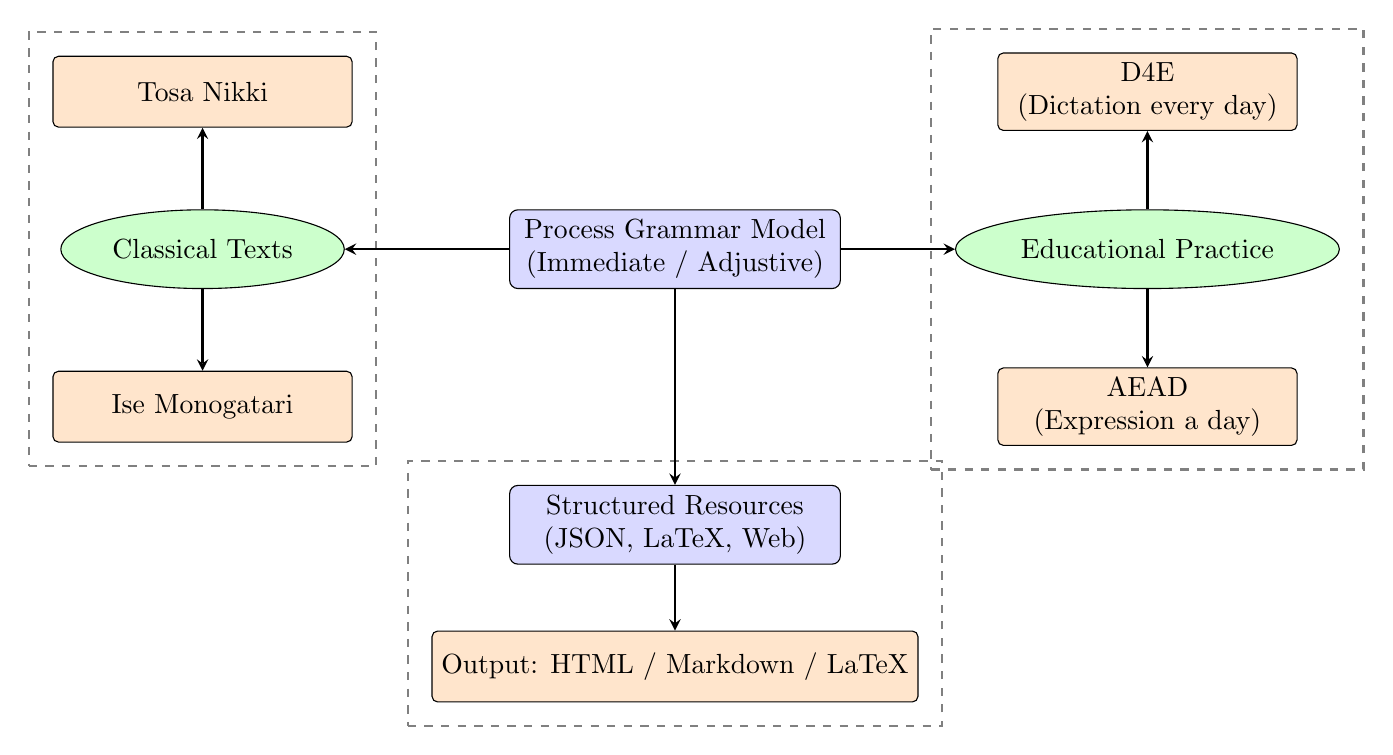
\begin{tikzpicture}[node distance=1cm and 2.5cm]

  % Central node
  \node (pgm) at (0,0) [mainnode] {Process Grammar Model\\(Immediate / Adjustive)};

  % Left side: Classical texts
  \node (classical) at (-6,0) [category] {Classical Texts};
  \node (tosa) at (-6,2) [subnode] {Tosa Nikki};
  \node (ise) at (-6,-2) [subnode] {Ise Monogatari};

  % Right side: Educational practice
  \node (education) at (6,0) [category] {Educational Practice};
  \node (d4e) at (6,2) [subnode] {D4E\\(Dictation every day)};
  \node (aead) at (6,-2) [subnode] {AEAD\\(Expression a day)};

  % Bottom side: Infrastructure
  \node (infra) at (0,-3.5) [mainnode] {Structured Resources\\(JSON, LaTeX, Web)};
  \node (output) at (0,-5.3) [subnode] {Output: HTML / Markdown / LaTeX};

  % Arrows from center
  \draw[connector] (pgm) -- (classical);
  \draw[connector] (pgm) -- (education);
  \draw[connector] (pgm) -- (infra);

  % Arrows from Classical
  \draw[connector] (classical) -- (tosa);
  \draw[connector] (classical) -- (ise);

  % Arrows from Educational
  \draw[connector] (education) -- (d4e);
  \draw[connector] (education) -- (aead);

  % Arrows from Infrastructure
  \draw[connector] (infra) -- (output);

  % Background groups
  \begin{pgfonlayer}{background}
    \node[draw=gray, dashed, thick, inner sep=0.3cm, fit=(tosa)(ise)(classical)] {};
    \node[draw=gray, dashed, thick, inner sep=0.3cm, fit=(d4e)(aead)(education)] {};
    \node[draw=gray, dashed, thick, inner sep=0.3cm, fit=(infra)(output)] {};
  \end{pgfonlayer}

\end{tikzpicture}
\end{document}
